
\section {Introduction:}


	The purpose of the literature survey is to get sufficient knowledge and to get familiar with the approaches, methods and strategies that are used before to solve the same problem on which we are going to work. In this paper, all approaches that we reviewed during our survey would be discussed. Moreover it will explain the limitations with the approaches and then it will answer the question ‘what is our strategy to solve this problem and why we choose it. \\
	In order to estimate the weight of the cattle by using the techniques of deep learning, computer vision and image processing, all research papers focuses on some of the common methods of pre-processing that can be used to segment out the region from the image. Once the image is segmented and separated from its background then some other advance techniques could be used for further calculation. All research papers that we read during our literature survey used different approaches to calculate the weight of the cattle. These approaches are discussed below in detail. \\
\section {Literature Survey Review:}
	
	During the survey, we reviewed the research papers which are summarized below separately. 
	
	\begin{center}
		\textbf{A measuring weight model of Timor’s Beef Cattle based on image}
	\end{center}

In this paper [3], the overall approach that is used to estimate the weight of cattle is by calculating the heart girth and body length of cattle. The overall structure of the approach that is used in this research paper is explained below by the block diagram. \\

\begin{figure}[h]
\centering
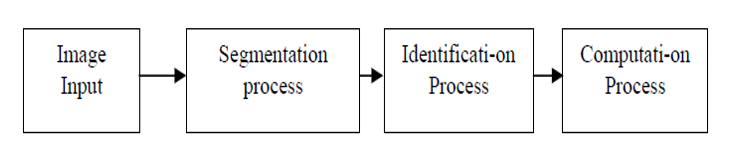
\includegraphics [scale=0.8] {flow_chart.PNG}
\caption{Diagram of image processing procedures}
\end{figure}



The paper didn’t say much about the procedure that is used to obtain the results but it explains the steps that they followed to get the results. According to their methodology they followed the following steps that are mentioned below.

\begin{enumerate}
	\item	Obtained or captured a digital image.
	\item	Performed image processing operations on image data.
	\item	Analyze and interpreted the image and use the results to get the body length, chest circumference and then use the standard formula to calculate the weight of cattle. 
	
\end{enumerate}

	The overall structure of the image processing method to get the weight of beef cattle can be demonstrated by the following block diagram [3]. \\
	


\begin{figure}[h]
\centering
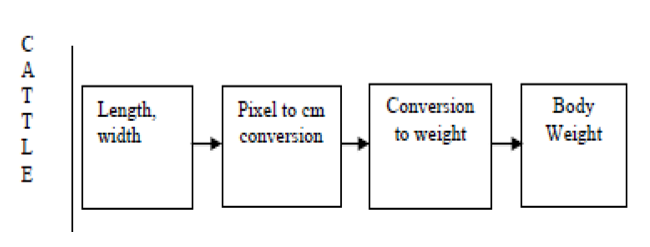
\includegraphics [scale=0.8] {blk_diagram.PNG}
\caption{Diagram of general process to Weighting the Cattle}
\end{figure}
	
	
	This paper cites some other research papers and explains the relationship between the body length and chest circumference. It gives reference to some formulas that can be used to determine the body weight of cattle. The author cites this research paper and according to Soeprapto [2], the body weight of cattle can be calculated by the formula:
	
	\begin{equation}\label{key}
		BW = \frac{BL + (CC)^{2}}{10840}
	\end{equation}
\textit{Where,}
\textit{BW} is the \textit{body weight} in kg \\ 
\textit{BL} is the \textit{body length} in cm \\ 
\textit{CC} is \textit{chest circumference} in cm \\

It cites another paper and says that according Schoorl written by Siregar [1], weight can be obtained by getting the physical dimensions of cattle. 
	
\begin{equation}\label{key}
BW  = \frac{(WoC + 22)^{2}}{100}
\end{equation}
Where, \textit{BW} is the \textit{body weight} in kg
\textit{WoC} is the \textit{width of chest} in cm


The author used the standardized formula based on the variables namely body length and chest width of cattle and obtained the results. He, in his paper claims that the results that were obtained by using this approach were not significantly different from the results of weighing using mechanical instrument [3]. 
\begin{center}
\textbf{	Weight Estimation Using Image Analysis and Statistical Modelling: A Preliminary Study}
\end{center}

The research was conducted previously on this topic and showed that there exists a correlation between the weight of the pig and physical features such as pig’s length or two dimensional area when viewed from above. This paper tries to find the correlation between the body weight of cattle and its physical features.\\

In the paper [4], the author automated the weight estimation system by using image processing techniques. The steps that are used in this approach as a part of image processing are following.

\begin{enumerate}
	\item 	Object Detection
	\item	Segmentation
	\item 	Filtering 
	\item	Feature Extraction 
	
\end{enumerate}


\textbf{Object Detection} \\

For the object detection, the author mentioned the calibration process that they used in their project. For calibration they set a fixed threshold. This threshold was determined by an offline calibration step. To complete this step, they took two images from a fixed camera rig; one image containing pig and other without pig (just of the background). These two images were used to locate the largest region of significant difference. Then they compared both images and based on the comparison results, a binary image was formed. Then a threshold was set based on brightness values in the binary image.  They author suggests a method to detect the pig in his paper. According to this paper [4], Pig detection could then be performed by sampling an image and comparing the measured brightness from the pixels in the defined detection region with the detection threshold. If a large percentage of pixels passed the test, then a pig was declared to be present and the image saved for further analysis. 

\begin{figure}[h]
\centering
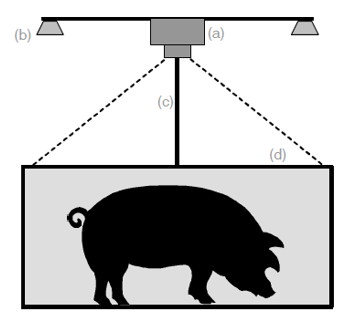
\includegraphics [scale=0.8] {camera_cali.PNG}
\caption{Camera and lighting setup}
\end{figure}


	
\textbf{Segmentation}

In the paper, fixed threshold method was used for segmentation. The author says that since the method was not entirely effective so in order to get the better results post filtering method was used to separate the object from the rest of the image. 
	
\textbf{Filtering}
	
Once the image is segmented, the post processing is required to clean up the segmented image. The post-processing involves two forms of filtering; median filtering and morphological filtering. A median filter is able to correct isolated segmentation errors, thereby “filling in” missed detections without causing great distortion to the image. It was also used to prevent the next process, image opening, from having a detrimental effect. After applying median filter image opening process was applied. 


\begin{figure}[h]
\centering
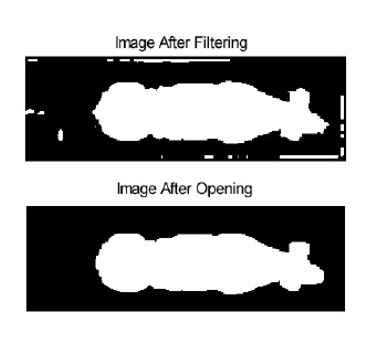
\includegraphics [scale=0.8] {image_open.PNG}
\caption{Image filtering and opening performed on the image of pig}
\end{figure}


	
\textbf{Feature Extraction}


After doing segmentation, the features were extracted to estimate the weight of cattle. The features that were employed in this study were area, length and spine length. The area of the object in pixels is trivially defined to be the sum of the binary pixel values over the whole image. This assumes that by this stage there will be only one contiguous region in the image.
The spine length was computed by isolating the largest branch in the skeleton and counting the number of pixels. The main branch was located by determining the location of junctions via a zero-crossing method [5]. 



\begin{figure}[h]
\centering
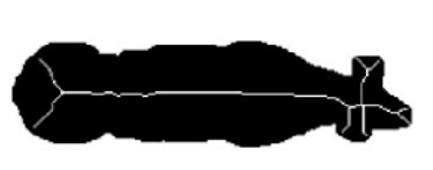
\includegraphics [scale=0.8] {skeleton.PNG}
\caption{Skeletonization performed on a segmented image}
\end{figure}


The length feature refers to the distance from the center of the pig’s neck to its tail. The position of the pig’s neck proved to be difficult to detect due to the unknown orientation of the pig’s head. It was decided to estimate the pig’s neck position as the point at which the main segment (referred to as the spine above) of the pig’s skeleton terminated. After skeletonization as above, the two endpoints of the spine were found [4]. \\
The “head” endpoint was deemed to be the one which gave rise to the most sub-branches, as the head was more topologically complex than the rump and usually produced a more structured sub-skeleton. The tail was assumed to be the most extreme pixel of the segmented image at the opposite end from the head. With these two data points the Euclidean distance could then be found, giving a close approximation of the length of the pig. Euclidean distance was appropriate since the pixel dimension ratio was one-to one [4]. \\
According to the author, the best results were obtained when using the neck-to-tail distance versus log weight (correlation coefficient 0.5640) and area versus weight (correlation coefficient 0.5295) to determine the weight. These correlation coefficients were both significant, having a probability of occurrence less than 1\%. The resulting linear weight prediction formulas achieve an average absolute error just under 5\% [4]. The author says, it confirms the claim that there exists a correlation between physical features and body weight. 

\begin{center}
	\textbf{Beef Cattle Weight Determine By Using Digital Image Processing} 
\end{center}


The body length, chest circumstance, height and width of the animal could be estimated.


\textbf{Image Preprocessing:}
The paper first did some image preprocessing depending on the image of cattle to make it segmented to do further calculation. 
Once the image is segmented it is divided into segmentation parts as shown in the figure below. [6]

\textbf{Suggested Segmentation Division:}

\begin{enumerate}
	\item Round and rear shank
	\item Sirloin, short loin, tenderloin, top sirloin, bottom sirloin, flank
	\item Rib and short plate
	\item Chunk, brisket and front shank
	


\begin{figure}[h]
\centering
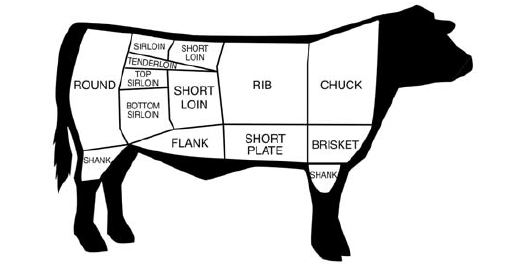
\includegraphics [scale=0.6] {beef.PNG}
\caption{Types of Beef}
\end{figure}
	
\end{enumerate}

\textbf{Methodology:}


\begin{enumerate}
	\item Localized Region Based Active Contour
	
	Segmentation method that minimizes curves in the segmentation process.
	
	\begin{equation}\label{key}
	E_{snake}= E_{internal} + E_{external} + E_{constraint}
	\end{equation}
	
	Make an initial contour surrounding the object, then with the energy of an object image (External) will cause the curve shrink and follow the pattern of the object. The curve can be moved closer towards the object and adjust the shape of the object because of the energy on the curve (Internal). Use active contour without edges which does not depend on the value of the gradient image as a condition to stop the contour changes. This model uses the average energy in the region. [6]
	

\begin{figure}[h]
\centering
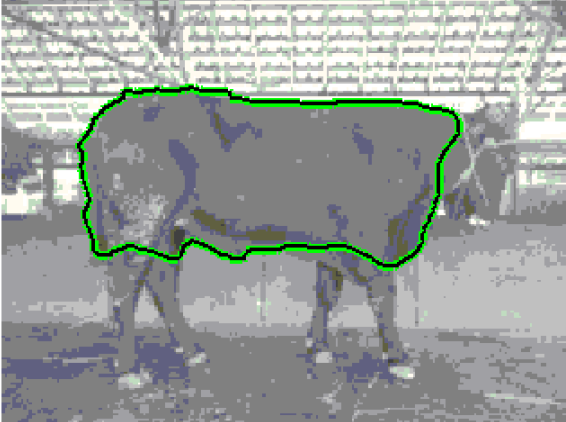
\includegraphics [scale=0.6] {contour.PNG}
\caption{Objects covered by the curve cantour}
\end{figure}
	
	\item Linear Regression
	
	Fitting a linear equation to observed data on two variables: explanatory variable, and dependent variable. Use scatter plot to determine whether or not there is a relationship between the variables of interest.[6]
	
	\item  Calculation Process
	
	To calculate the weight of each part, the part of side picture of cattle feature will be regressed with chest feature data.[6]
	
	The results that were obtained from this approach were as follow. 
	\begin{enumerate}
		\item	73.213\% accurate system;
		\item	Accuracy between segmented object and without segmentation is the same because of anatomical shape. 
	\end{enumerate}
	
	
\end{enumerate}

\begin{center}
		\textbf{Estimation of Calf Weight from Fixed Point Stereo Camera Images using 3D Successive Cylindrical Model}
\end{center}


In order to improve productivity, the objective is to simplify the estimation of calf weight. In this paper, method to estimate weight by three-dimensional model of cattle shape using stereo images is proposed. This enables to solve the problem that requires no special environment to shoot images only from above in the previous work. Moreover, it can mitigate the issue of the posture of cattle by grasping it three-dimensionally. In the proposed method, firstly, the stereo camera is created by fixing two network cameras. The image of the calf is taken by these cameras, and the stereo matching method is applied to the captured image to calculate three dimensional coordinates. Next, only the body is modelled because chest girth and waist girth have the highest correlation with weight. Since the body has a rounded shape, a three-dimensional successive cylindrical model is used. Weight estimation by using the linear regression equation between the volume of the obtained three-dimensional successive cylindrical model is obtained and the weight measured manually. [7]

\textbf{Basic Information of Cattle Body and Extraction of Body Parts Data}


Two fixed network cameras shoot motion images of calves. These motion images are divided into frames and analysed as static images. The image can be used as a stereo image by calibration of cameras. In stereo matching, the distance between the camera and the target object is kept constant. This distance depends on the size of the target object. In this paper, the distance ranged from 1 to 3 meters. [7]




\begin{figure}[h]
\centering
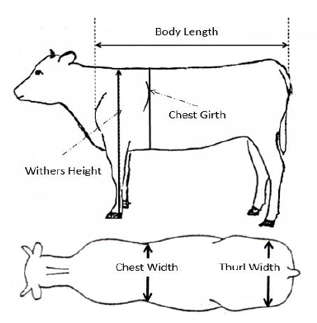
\includegraphics [scale=0.8] {parts}
\caption{Each parts of cattle body}
\end{figure}


Two methods are used to extract body parts of the cattle from the stereo images. First method is background subtraction method where the background image is taken in advance. Second method is using parallax values obtained from the stereo matching method.
Both of these methods output mask images. The common part of these two mask images is taken to extract the cattle body. This process eliminates the noise. The output image is converted to binary to give cattle body in white and remaining in black. 




\begin{figure}[h]
\centering
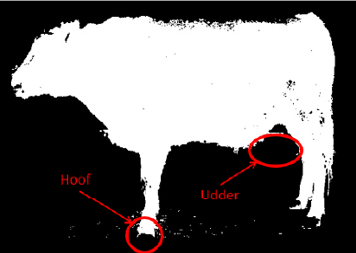
\includegraphics [scale=0.8] {bin_img.PNG}
\caption{Binary image of cattle}
\end{figure}


\textbf{Modeling Body of Cattle}

Measuring chest girth precisely is difficult so it model the entire body using a successive cylindrical model to find correlation with weight. Three-dimensional point cloud data is calculated from stereo images using the stereo matching method. Surface of cattle is smooth with little change in colour, therefore the errors are high and volume cannot be determined precisely. Therefore, we attempt to model it by using a simple and fixed three-dimensional model. [7] A cylindrical model is chosen since it best models the rounded shape of the cattle body. It is necessary to divide the body into several parts in order to change the radius of the cylindrical model according to the position in the x direction of the body. [7]




\begin{figure}[h]
\centering
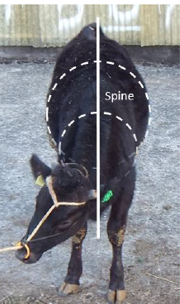
\includegraphics [scale=0.8] {front.PNG}
\caption{Cattle from above}
\end{figure}


The radius of the cylindrical model is determined by using the circle closest to the point cloud data. This enables to detect the body shape while reducing errors. To develop the circle nearest to the point cloud data, a circle fitting using a generalized Hough transform is employed. 




\begin{figure}[h]
\centering
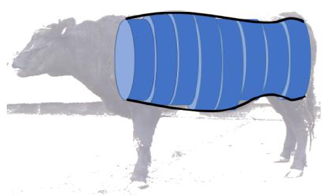
\includegraphics [scale=0.8] {spiral.PNG}
\caption{Successive cylindrical model}
\end{figure}


First, when comparing the cases where the body is divided and not divided, the correlation coefficient and the average error are better when divided. Then, comparing the case where each result was individually examined and the volume was averaged, all of the result was better when the volume was averaged. Thus, it verified the effectiveness of slicing the image of the body with the proposed method and to shoot and use multiple images of the same cattle. [7]
The experimental results have revealed the following: 

\begin{enumerate}
	\item There is a correlation between weight and volume obtained by modeling the body. 
	\item The proposed method that models by slicing the image of the body is highly effective. 
	\item There is a possibility to improve accuracy of weight estimation by using multiple stereo images
	
\end{enumerate}

\begin{center}
	\textbf{	Weight Estimation through Image Analysis}
\end{center}

In this paper [9], image segmentation based technique has been used to segment out the region from the image and then using the dimension of the image object weight has been calculated using density based formula. According to the author, it was observed through this experimental process, results were 92\%-94\% accurate. [9] \\
The strategy that is used in the paper can be understood by the following flow chart diagram.



\begin{figure}[h]
\centering
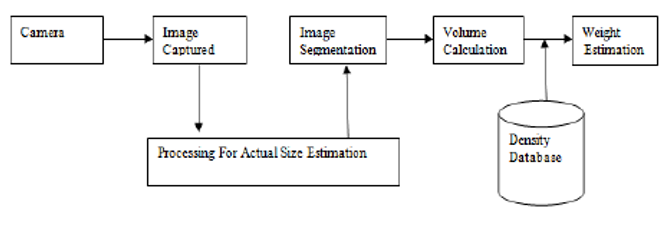
\includegraphics [scale=1.0] {flowChart.PNG}
\caption{Process Flow Chart}
\end{figure}



The propose strategy in paper [9] consists of the following steps. 

\begin{enumerate}
	\item 	Pre-Processing
	\item 	Image Segmentation
	\item 	Volume Calculation 
	\item 	Mass Calculation
\end{enumerate}

\textbf{Pre-Processing}\\
The image is a 2D array which consists of finite and discrete pixel values. In order to segment out the foreground object (cattle in this case) from background some pre-processing is required. In pre-processing phase the image is downscaled for faster computation. The pre-processed image is segment using K-means clustering algorithm to extract the object from the image. The image is divided in which subtraction of the image comprising the object cluster is used for further processing. [9]


\textbf{Image Segmentation}

In this phase, the image that was obtained from the pre-processing step is then segmented using watershed segmentation algorithm to extract the object from the image.  

The paper [9] explains the method that is used to calculate the volume in detail. Let f(x, y) be the input from the front view and s(x, y) be the input from the side view which is then preprocessed to get f`(x, y) and s`(x, y). These preprocessed images are passed through the segmentation function, as mentioned above, to get clustered images of front and side view, that is g(x, y) and h(x, y) respectively. The subsection of g(x, y) and h(x, y) containing the object’s cluster. The grid area technique is applied on the segmented images. The M x N subsection is selected for grid area calculation. The subsection consists of object’s cluster O and background cluster G is further divided into smaller grid of size m x n. The M x N is then iterated for every grid and for each grid if more than 50\% pixels in the grid belong to object’s cluster O then the grid is considered to be a part of the object’s cluster. The iteration gives the total number of grids belonging to O, that is, O[n]. The count O[n] is stored in a vector for every column in the grid array. The grid area returns two vectors, $C_{ocside}$ for side image and $C_{ocfront}$ for front image. After applying this technique, the following cases might arises. 


\begin{enumerate}
	\item The vector have equal dimensions 
	\item The vector have unequal dimensions
	
\end{enumerate}

\textbf{Volume Calculation}

If the dimension are not equal then extra elements from the larger vector are removed and average of these elements is inserted back into vector. 
Volume can be calculated using the following formula. 

\begin{equation}\label{key}
Volume = (\sum_{i=0}^{n} C_{ocfront} (i) + C_{ocside}(i)) * V_{grid} * sf^{3}
\end{equation}
$ Where,  V_{grid} =$ \textit{Volume of the grid cube}\\
$sf = \textit{Scaling Factor} $
\\

\textbf{Mass Calculation}

Using the volume of object obtained from the above mentioned process, the mass can be calculated as follow.

\begin{equation}\label{key}
Mass = Density * Volume
\end{equation}

\pagebreak 

\begin{center}
\textbf{Learning Deep Features for Discriminative Localization}
\end{center}


\paragraph{}In this research paper, we visit the global average pooling layer and shed light on how it explicitly enables the convolutional neural network (CNN) to have 
remarkable localization ability despite being trained on imagelevel labels. While this technique was previously proposed as a means for regularizing training, 
we see that it actually builds a generic localizable deep representation that exposes the implicit attention of CNNs on an image. Despite the apparent simplicity of global average pooling, we are able to achieve 37.1\% top-5 error for object localization on ILSVRC 2014 without training on any bounding box annotation. We can see in a variety of experiments (given below) that the network is able to localize the discriminative image regions despite just being trained for solving classification. [8]

\begin{figure}[h]
\centering
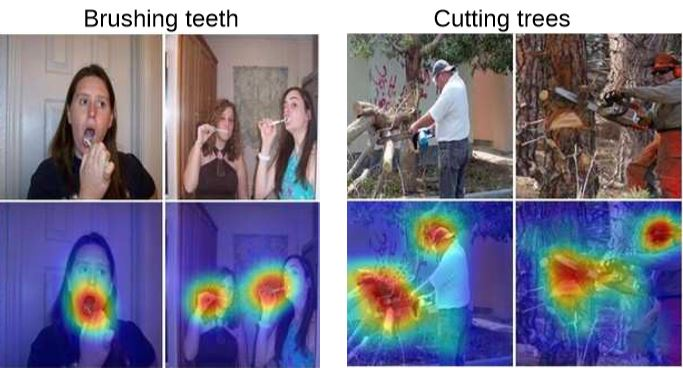
\includegraphics [scale=0.8] {Figure1.jpg}
\caption{Simple modification of the global average pooling layer combined with our class activation mapping}
\end{figure}

\paragraph{}The final output above is called Class-Activation-Map(CAM). It is actually the regions of the image that are the deciding factors during classification i.e. 
Discriminative-Regions (DR). These maps are calculated by first finding the node with the highest classification score and then finding the weights that connect 
the neurons from Global Average Pooling (GAP) layer to the final layer (classification layer). We can then find the linear combination of these weights and feature maps obtained from the last convolutional layer to find the CAM. The figure below illustrates that.

\begin{figure}[h]
\centering
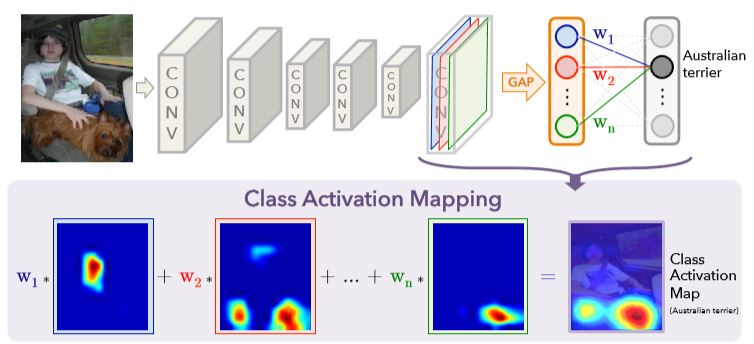
\includegraphics [scale=0.8] {Figure2.jpg}
\caption{Class Activation Mapping: the predicted class score is mapped back to the previous convolutional layer to generate the classactivation maps (CAMs). The CAM highlights the class-specific discriminative regions}
\end{figure}

The results shown are evident that localization problems(with reliable results) can be solved by using a vanilla CNN without going into the complexity of object detection.[8]



\section{Conclusion}

The research papers we reviewed did not incorporate the depth information which in our case would greatly increase accuracy. To counter this, we explored 3 different approaches in order to predict the weight of the cattle as accurately as possible.

\subsection{Approaches}

\subsubsection{Automated Heart Girth Measurement Where depth is Fixed}

The heart girth measurement is the most reliable technique of estimating the weight. In this approach, we take two variables; Heart Girth and the Body Diagonal. We assume that the depth of the animal i.e the distance of the animal from the camera is either known or fixed. We take two images, the front view and the side view. The width of the animal is determined from the front view. To get both the variables, we convert the number of pixels in the image to real-world measurements using the formula described in curve length estimation section. 

The following vectors are obtained from the images:

\begin{center}
$\vec H = [p1, p2, p3 ... pN]$\\
$\vec D = [dp1, dp2, dp3 ... dpN]$
\end{center}
Where H = Heart Girth Pixel Vector and D = Diagonal Pixel Vector.

\subsubsection{Heart Girth Measurement with Per-Pixel Depth}

This approach builds upon the previous approach. We take the same variables i.e the Heart Girth and the Body Diagonal. This method however requires only 1 image; the side view of the animal. We find the inner and outer bounding boxes around the required parts of the animal. The curvature of the animal is estimated using the per pixel depth information. 

The following vectors are obtained from the images:

\begin{center}
$\vec Hp = [p1, p2, p3 ... pN]$\\
$\vec Dp = [dp1, dp2, dp3 ... dpN]$

\end{center}

Where H = Heart Girth Depth per Pixel Vector and D = Diagonal Depth per Pixel Vector.



\subsubsection{Curve Length Estimation:}

In the above mentioned approaches the final result we get is a bounding box from our core component using our deep learning model which encapsulates the information of body length in the diagonal and heart girth measurements in height of the box. Since these values are just only represented by two pixel coordinates top-left and bottom right. As mentioned earlier to get the measurements accurate we have to incorporate the depth information. Since we have depth map and RGB image of same dimensions and from same camera we can safely map this bounding box to depth image as well. 

Once we have a this image box on depth image we will extract out the vector of pixels from the heart girth line of the bounding box and diagonal vector from pixels starting from bottom left and the top right  point in this image.
Once we have these two vectors we can convert it into real world measurements using the procedure defined below in Appendix.B, Math section. 

 




